\documentclass{standalone}
\usepackage{tikz}
\begin{document}
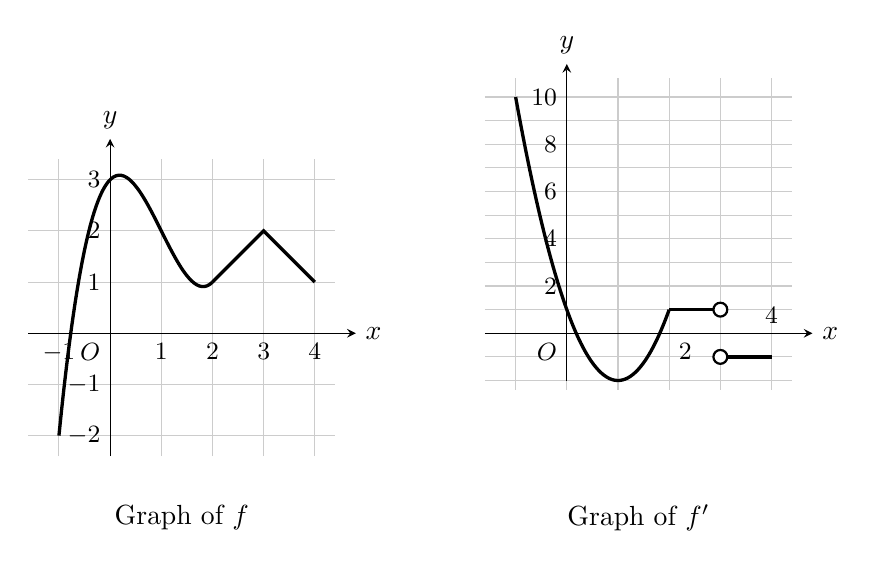
\begin{tikzpicture}[>=stealth]
  % Left panel: graph of f on [-1, 4]
  %   f(x) = x^3 - 3x^2 + x + 3 on [-1, 2]  (f(-1) = -2, f(0) = 3, f(1) = 2, f(2) = 1)
  %   f(x) = x - 1 on [2, 3], f(x) = 5 - x on [3, 4]
  \begin{scope}[x=0.65cm, y=0.65cm]
    \foreach \x in {-1,...,4} { \draw[gray!40] (\x,-2.4) -- (\x,3.4); }
    \foreach \y in {-2,...,3} { \draw[gray!40] (-1.6,\y) -- (4.4,\y); }
    \draw[->] (-1.6,0) -- (4.8,0) node[right] {$x$};
    \draw[->] (0,-2.4) -- (0,3.8) node[above] {$y$};
    \foreach \x in {-1,1,2,3,4} {
      \node[below, font=\small] at (\x,0) {$\x$};
    }
    \foreach \y in {-2,-1,1,2,3} {
      \node[left, font=\small] at (0,\y) {$\y$};
    }
    \node[below left, font=\small] at (0,0) {$O$};
    \draw[very thick, domain=-1:2, samples=60, smooth]
      plot (\x, {\x*\x*\x - 3*\x*\x + \x + 3});
    \draw[very thick] (2,1) -- (3,2) -- (4,1);
    \node at (1.4,-3.6) {Graph of $f$};
  \end{scope}

  % Right panel: graph of f' on [-1, 4]
  %   f'(x) = 3x^2 - 6x + 1 on [-1, 2]  (f'(-1) = 10, f'(0) = 1, f'(1) = -2, f'(2) = 1)
  %   f'(x) = 1 on [2, 3), f'(x) = -1 on (3, 4]; f'(3) is undefined
  \begin{scope}[xshift=5.8cm, x=0.65cm, y=0.3cm]
    \foreach \x in {-1,...,4} { \draw[gray!40] (\x,-2.4) -- (\x,10.8); }
    \foreach \y in {-2,...,10} { \draw[gray!40] (-1.6,\y) -- (4.4,\y); }
    \draw[->] (-1.6,0) -- (4.8,0) node[right] {$x$};
    \draw[->] (0,-2) -- (0,11.4) node[above] {$y$};
    \foreach \y in {2,4,6,8,10} {
      \node[left, font=\small] at (0,\y) {$\y$};
    }
    \node[below right, font=\small] at (2,0) {$2$};
    \node[above, font=\small] at (4,0) {$4$};
    \node[below left, font=\small] at (0,0) {$O$};
    \draw[very thick, domain=-1:2, samples=60, smooth]
      plot (\x, {3*\x*\x - 6*\x + 1});
    \draw[very thick] (2,1) -- (3,1);
    \draw[very thick] (3,-1) -- (4,-1);
    \draw[thick, fill=white] (3,1) circle (2.5pt);
    \draw[thick, fill=white] (3,-1) circle (2.5pt);
    \node at (1.4,-7.8) {Graph of $f'$};
  \end{scope}
\end{tikzpicture}
\end{document}
